In addition to the results of the models discussed above, we can look at some summary statistics of the data to give us some insight into the plight of graduate students across the US.

Firstly, we can look at total number of thesis submissions on the ProQuest Thesis and Dissertation Database. This is shown in Figure~\ref{fig:pub_theses}.

\begin{figure}[H]
  \centering
  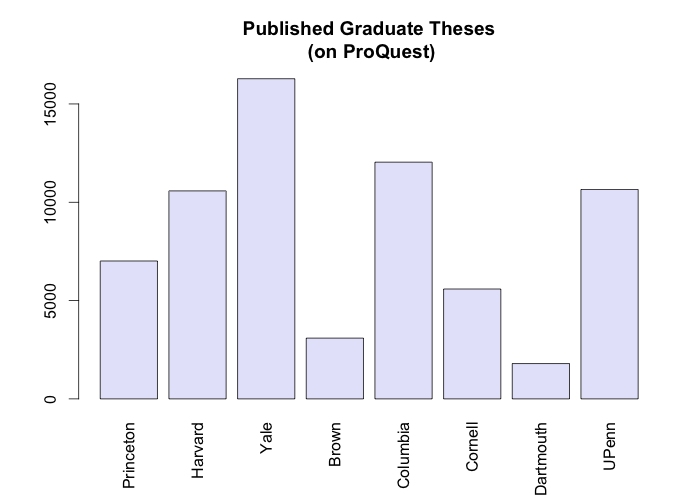
\includegraphics[width=0.5\textwidth]{img/pub_theses.png}
  \caption{Number of published graduate theses in ProQuest database}
  \label{fig:pub_theses}
\end{figure}

In Figure~\ref{fig:ack_lengths}, we can see that acknowledgement lengths drop off according to something akin to a power law, with a median length of around 400 words.

\begin{figure}[H]
  \centering
  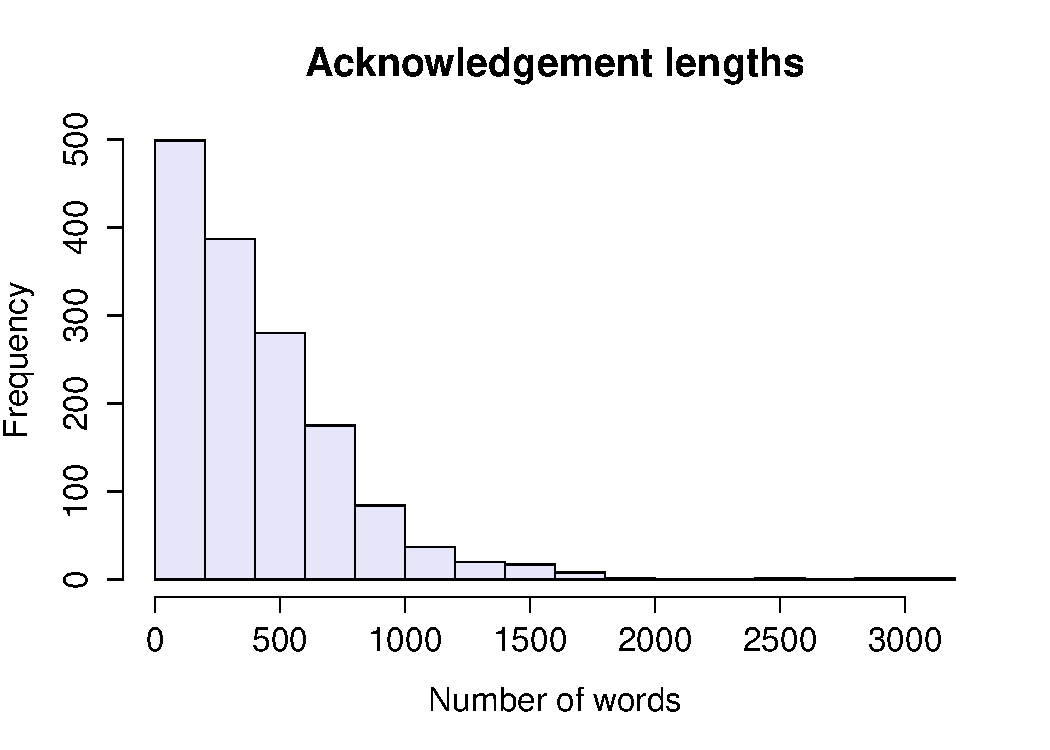
\includegraphics[width=0.5\textwidth]{img/ack_lengths.pdf}
  \caption{Acknowledgement lengths in graduate theses}
  \label{fig:ack_lengths}
\end{figure}

Examining the results of our models, we the table of fitted values for the university-conditional Gaussian positivity model is shown in Figure~\ref{fig:gaussian_model}. This provides one a plausible ranking of Ivy League universities by student satisfaction. Note, however, that the standard deviation of each university's positivity ratio is comparable to the inter-university positivity ratio differences, meaning that we cannot claim this ordering is statistically significant. This suggests that we may need to subclass the data within universities (by department, or field, most likely) in order to get clearer results. While the number of documents we collected was insufficient for this purpose, it would only be a matter of time and patience to collect a substantially larger corpus with which to work.

\begin{figure}[hH]
  \centering
  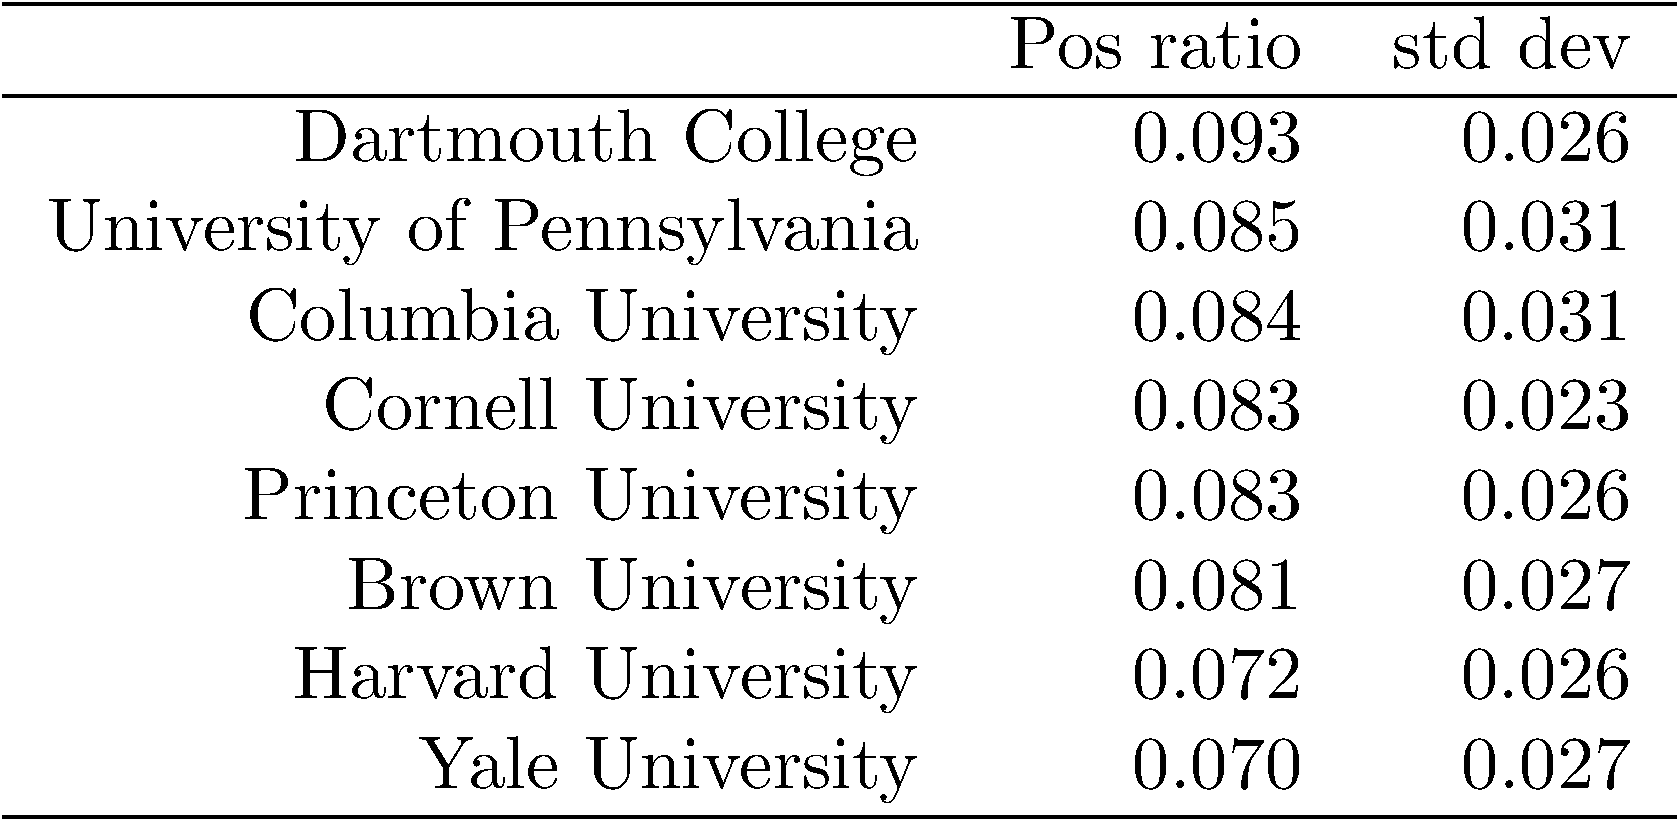
\includegraphics[width=0.5\textwidth]{img/gaussian_model.pdf}
  \caption{Fitted parameters to the university-conditional Gaussian positivity model}
  \label{fig:gaussian_model}
\end{figure}

The Naive Bayes classifier gave an accuracy of 72\% in predicting whether a student would fall in the top or bottom 50\% of positivity ratios, given the z-scored values for the university, the field (either biomedical sciences, humanities or sciences), the total number of negative words and the word count. The confusion matrix for the Naive Bayes classifier is included in Figure~\ref{fig:conf_matrix}.

\begin{figure}[hH]
  \centering
  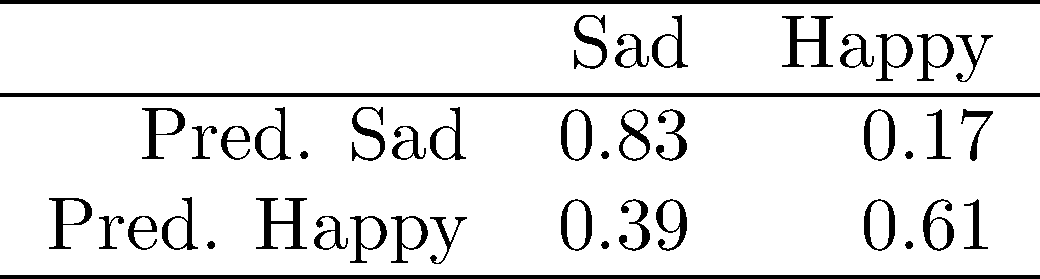
\includegraphics[width=0.5\textwidth]{img/conf_matrix.pdf}
  \caption{Confusion matrix for Naive Bayes classifier. Categories correspond to top and bottom 50\% of positivity ratios.}
  \label{fig:gaussian_model}
\end{figure}

Lastly, the rankings of positivity by field were:
\begin{enumerate}
  \item Sciences (mean 8.4\% positivity ratio)
  \item Biomedical sciences (mean 8.3\% positivity ratio)
  \item Humanities (mean 7.6\% positivity ratio)
\end{enumerate}
It is an open question as to whether these inter-subject differences are affected by differences in thesis conventions between subject areas.